%!TEX root = kPtx_paper.tex
\section*{Results}

\begin{figure}
	\centering
	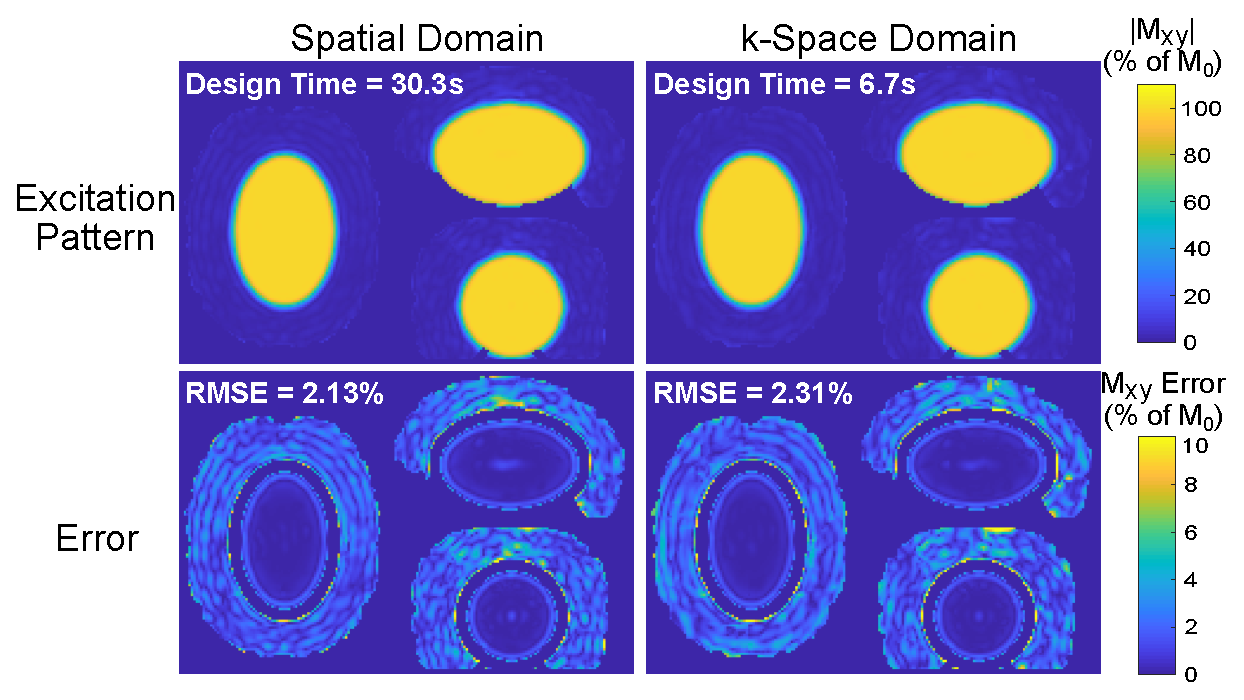
\includegraphics[width=\textwidth]{ErrorMap}
	\caption{\textcolor{red}{WAG: I think this is the figure that your example in Github should replicate.}
	Normalized excitation patterns (top row) and error maps (bottom row) in central axial, sagittal and coronal slices 
	for k-space domain (left) and spatial domain designs (right).}
	\label{fig:ErrorMap}
\end{figure}
Figure \ref{fig:ErrorMap} shows simulated excitation patterns and error maps for the reference spatial and k-space domain designs. 
Both designs were performed with 16 parallel threads and the 64$\times$64$\times$48 grid size (3 mm isotropic resolution), 
and the excitation patterns were evaluated against the target pattern on a 128$\times$128$\times$96 grid size (1.5 mm iso-resolution). 
The k-space domain design used patch and inclusion widths of 4.
The calculated root-mean-squared errors (RMSEs) were 2.42\% (spatial domain) and 2.68\% (k-space domain), 
respectively. 
For both design methods, most of the errors appeared at the edges of the transition band, 
and errors elsewhere were lower than 5\% of the target flip angle. 
This indicates uniform inner volume excitation while maintaining the outer volume intact. 
The parallelized k-space domain design required 2.9 seconds computation versus 31.8 seconds for the spatial domain method, a 91\% decrease.

\begin{figure}
	\centering
	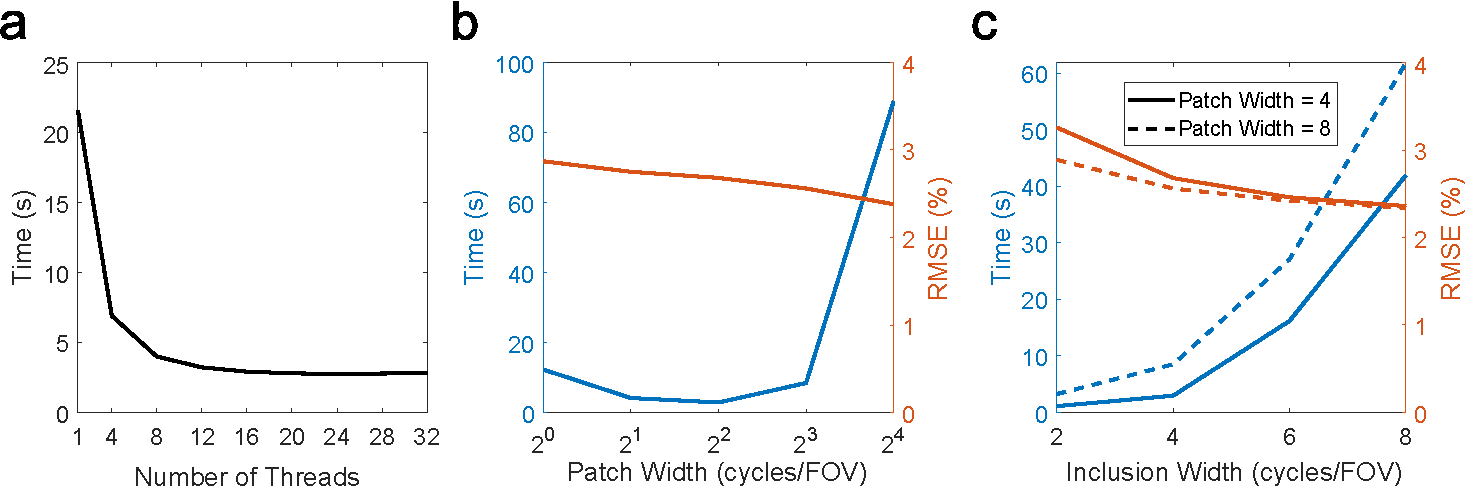
\includegraphics[width=\textwidth]{ComputationTime}
	\caption{(a) k-Space computation time versus number of parallel threads, for patch and inclusion widths of 4 cycles/FOV. 
	(b) Computation time (blue axis) and RMSE (red axis) versus patch width, for an inclusion width of 4 cycles/FOV and 16 threads. 
	(c) Computation time (blue axis) and RMSE (red axis) versus inclusion width, for patch widths of 4 and 8 cycles/FOV, and 16 threads.}
	\label{fig:ComputationTime}
\end{figure}
\subsection*{k-Space Algorithm Parameters}
Figure \ref{fig:ComputationTime}a plots mean computation time versus number of parallel threads,
holding the patch and inclusion widths fixed at 4 cycles/FOV. 
The computation time decreased rapidly with increasing thread number up to 12 threads, 
and then plateaued, likely due to the overhead involved in initiating threads after that point.
Based on this result, the number of threads was held fixed at 16 for subsequent designs when off-resonance was not compensated.

\par Figure \ref{fig:ComputationTime}b plots mean computation time and RMSE with different patch widths. 
The computation time decreased up to a patch width of 4 cycles/FOV (corresponding to $4^3 = 64$ simultaneously solved columns of $\bm{W}$) 
and then increased sharply for larger patch widths. 
RMSE decreased slowly as the patch width increased since the number of excitation trajectory points included in the calculation of weights for each 
target point increases on average (and especially for target locations in the middle of each patch) as the patch width increases, 
even when the inclusion width stays fixed.
Based on this result, a patch width of 4 cycles/FOV was used for subsequent designs.

\par Figure \ref{fig:ComputationTime}c plots mean computation time and RMSE with different inclusion widths. 
The solid lines and dashed lines were obtained with patch widths of 4 and 8 cycles/FOV, respectively. 
Computation time increased and error decreased with increasing inclusion width,
since more excitation trajectory points were included in each target location's calculation for increasing inclusion width,
corresponding to an increased $\bm{S}^H\bm{S}$ matrix size. 
The RMSE was only slightly lower for a patch width of 8 versus 4 cycles/FOV, 
but the computation time was much higher for 8 cycles/FOV, across all inclusion widths. 
The knees in the curves occurred approximately at an inclusion width of 4 cycles/FOV,
so this value was used in subsequent designs. 

\par Table \ref{fig:wsize} lists the size of the final matrix $\bm{W}$ in gigabytes,
versus inclusion width.
As inclusion width increases, more excitation trajectory points are used in the solution of the weights for each target location,
until the entire trajectory is used for each location (Inclusion width = $\infty$ in the table),
corresponding to a full solution. 
With the inclusion width of 4 cycles/FOV used here, 
the matrix size was 98\% smaller than that of a full solution.  

\begin{figure}
\centering
\begin{tabular}{c | c}
Inclusion Width & $\bm{W}$ Matrix Size (GB) \\
\hline
$\infty$ & 24.4 \\
8 & 2.73 \\
6 & 1.37 \\
4 & 0.53 \\
2 & 0.14
\end{tabular}
\caption{$\bm{W}$ matrix sizes in gigabytes (GB) versus inclusion width in cycles/FOV. 
An inclusion width of $\infty$ corresponds to a full matrix solution.}
\label{fig:wsize}
\end{figure}

\begin{figure}
	\centering
	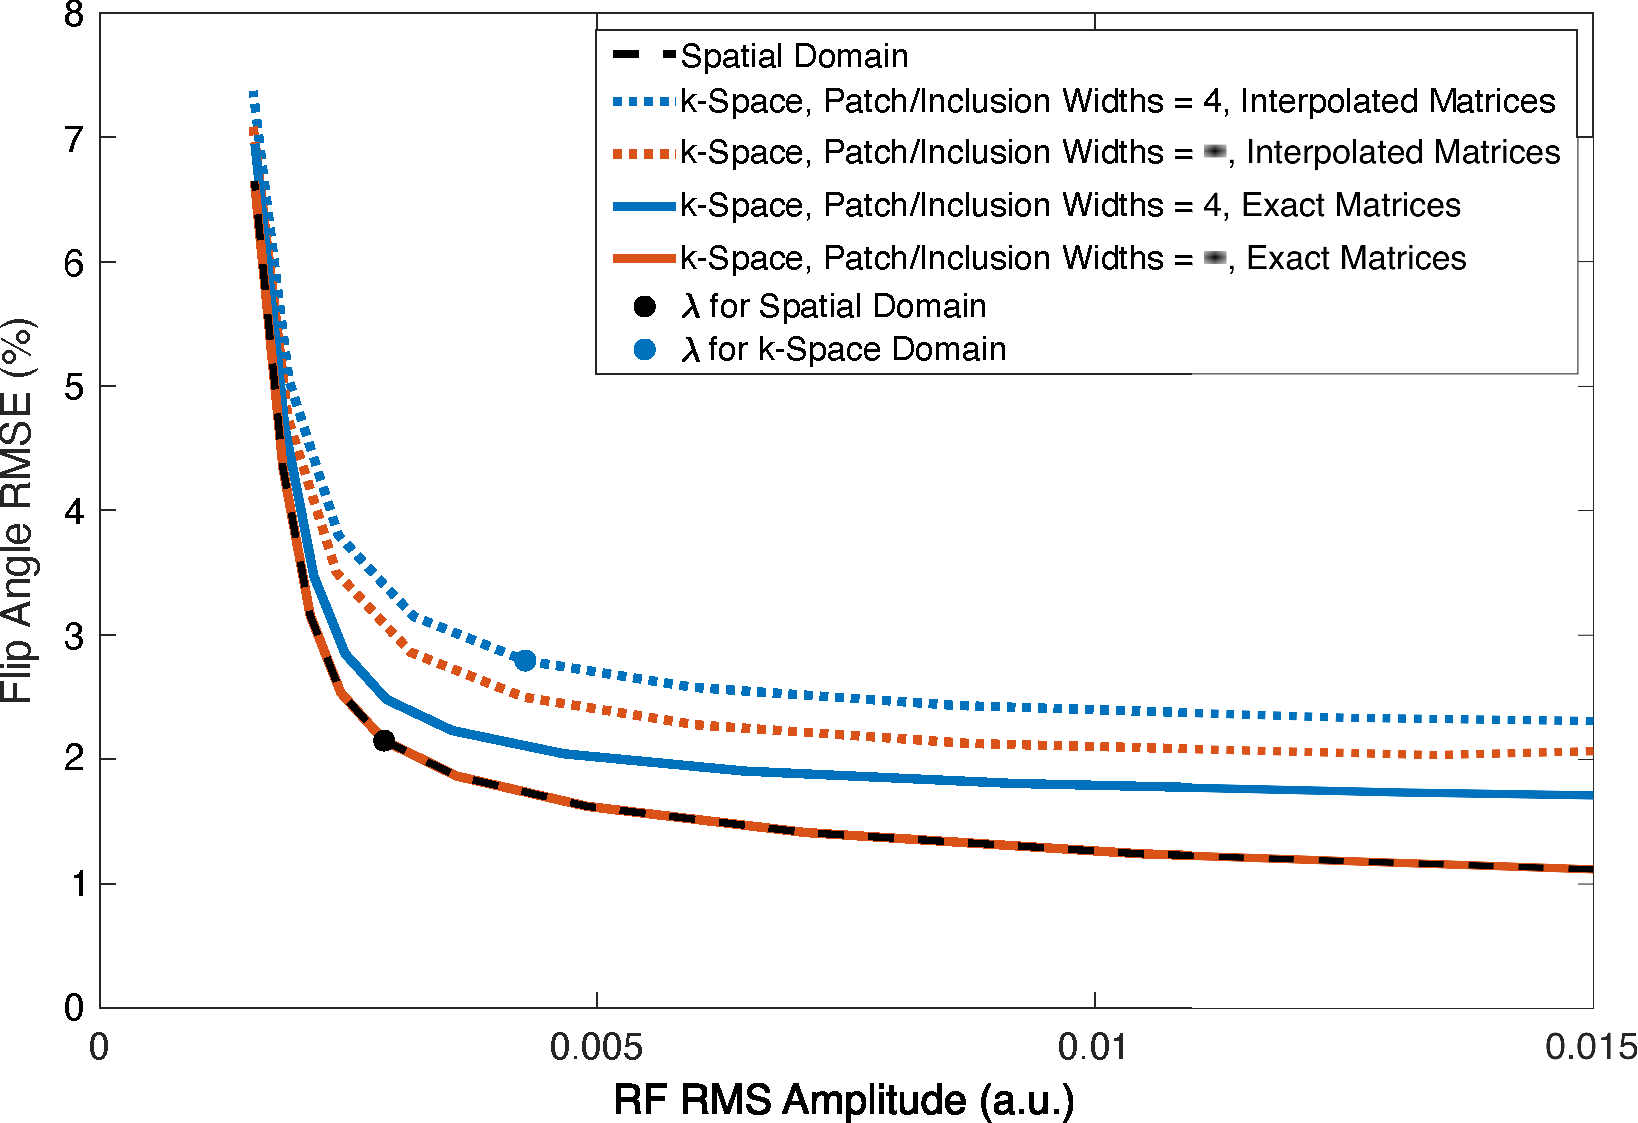
\includegraphics[width=\textwidth]{L_curve}
	\caption{L-curves for spatial domain and k-space domain pulse designs, 
	repeated across five orders of magnitude of the methods' Tikhonov regularization parameters.
	The k-space domain designs were repeated using patch and inclusion widths of four versus solving for the entire domain at once (`Patch / Inclusion Width = 4' versus `Full Patch'),
	and using $B_1^+$ map product interpolation versus phase modulation to each trajectory location (`Interpolated $\bm{S}^H\bm{S}$ Matrices' versus
	`Exact $\bm{S}^H\bm{S}$ Matrices').}
	\label{fig:LCurves}
\end{figure}

\subsection*{L-Curves}


\begin{figure}
	\centering
	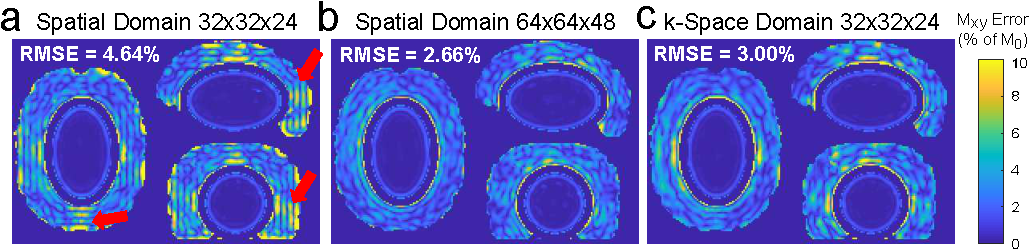
\includegraphics[width=\textwidth]{GibbsRinging}
	\caption{Normalized error maps and RMSE for \textbf{(a)} spatial domain design and \textbf{(c)} k-space domain design with 6 mm iso-resolution, 32$\times$32$\times$24 design grid. Red arrows indicate the Gibbs ringing in low-resolution spatial domain design. \textbf{(b)} Normalized error map for spatial domain design with 3 mm iso-resolution, 64$\times$64$\times$48 design grid.}
	\label{fig:GibbsRing}
\end{figure}

\subsection*{Gibbs Ringing}
Figure \ref{fig:GibbsRing}a\&c show the results of the  low-resolution designs using k-space domain method and the spatial domain method. The result of the high-resolution design of the spatial domain is also shown in Figure \ref{fig:GibbsRing}b. All three designed were done with a excitation trajectory that matches the 6 mm iso-resolution. The red arrows indicate the Gibbs ringing in the low-resolution spatial domain design, that can only be suppressed with high-resolution spatial domain design. However, the k-space domain design, although also low-resolution, is insensitive to this problem. Furthermore, the ripple pattern in the low resolution k-space design matches the high-resolution spatial design. Looking from a spatial domain point of view, the Gibbs ringing was caused by the lack of ability to observe the ringing with low-resolution. Looking from a k-space domain point of view, the Gibbs ringing was due to "wrap back" of the k-space FOV. When the spatial resolution is low the k-space FOV is small, and therefore the RF samples at one end of the trajectory can incorrectly "reach" and affect the k-space points at the other end of the k-space FOV in a circulation shift fashion. However, for the k-space domain design, even with low resolution, there is no k-space "wrap back" because the incorporated trajectory points are explicitly specified. Particularly, for the instance problems whose patches are at the edges of the k-space FOV, the excitation trajectory points at the other ends of the k-space FOV will not be incorporated into the design.    


\begin{figure}
	\centering
	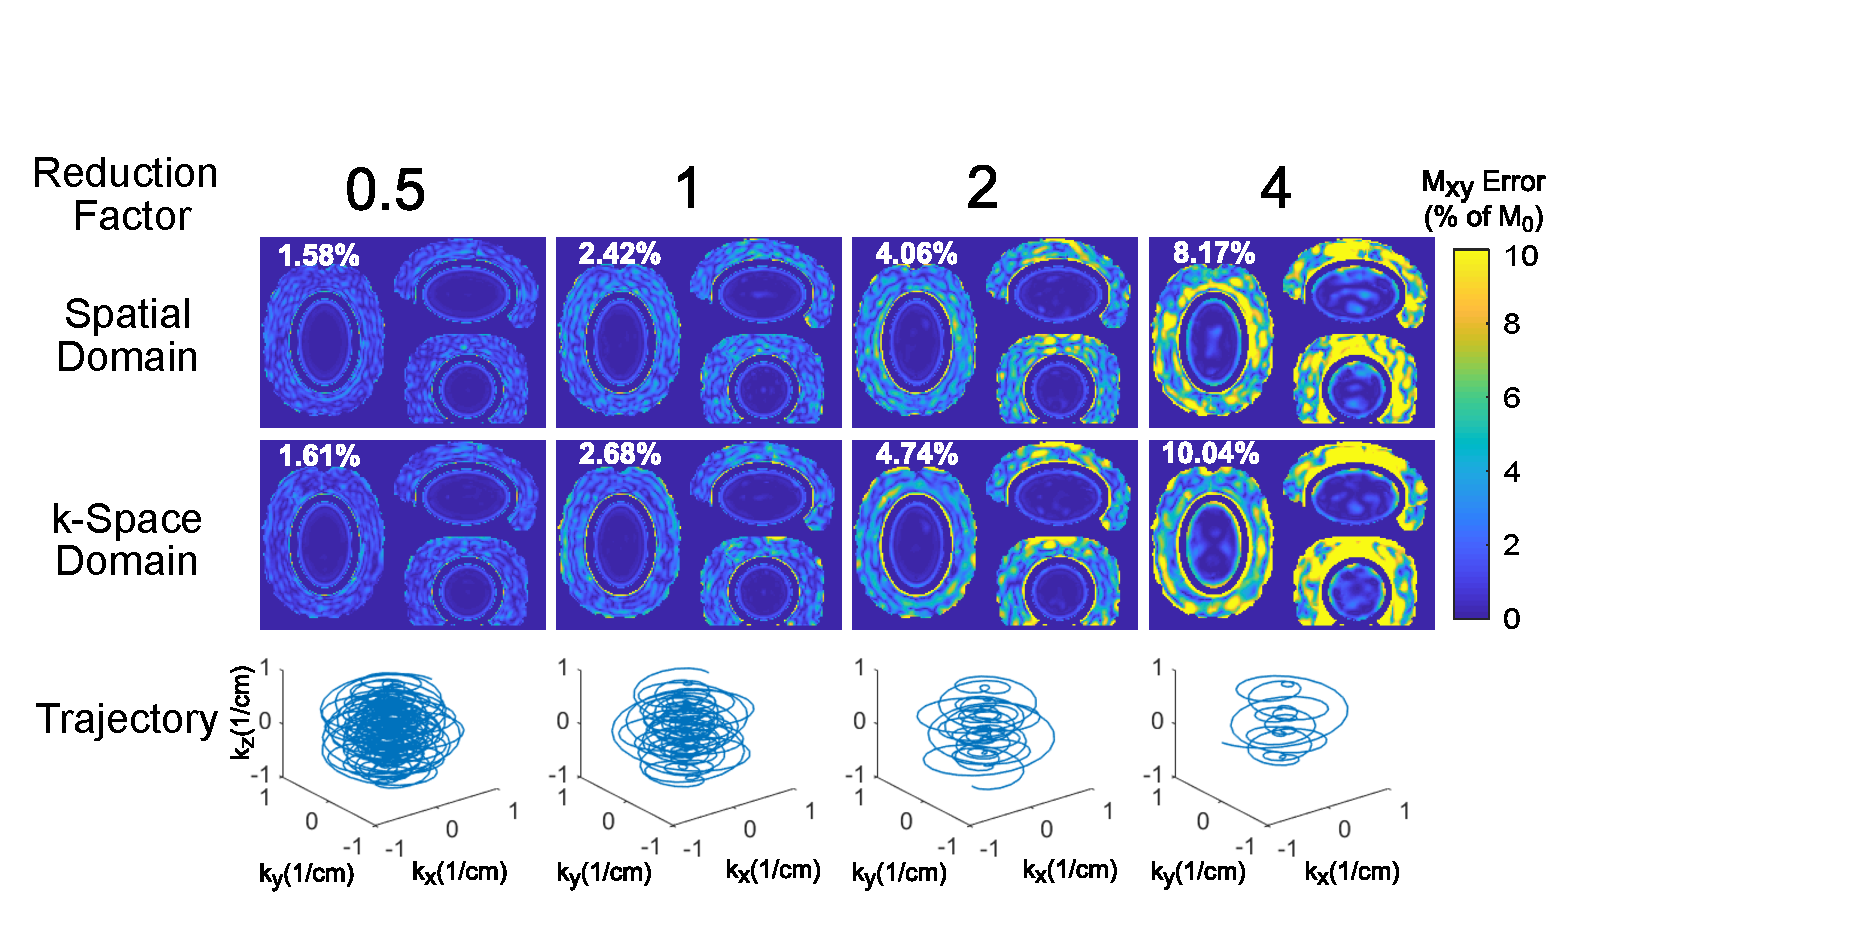
\includegraphics[width=\textwidth]{ReductionFactor}
	\caption{Normalized error maps and RMSE for spatial domain design (first row) and k-space domain design (second row), 
	using excitation k-space trajectories with different reduction factors (third row).
	The reduction factors are referenced to the 10 ms trajectory in Figure \ref{fig:Target} (second column).}
	\label{fig:kspace_PTX_Acceleration}
\end{figure}

Figure \ref{fig:kspace_PTX_Acceleration} shows a comparison between the performance of spatial domain design (first row) and k-space domain design (second row) regarding undersampled excitation trajectories (third row) with different reduction factors. Both design methods had larger errors when the excitation k-space was less densely traversed. The k-space domain design provided similar error maps and practically equal RMSE. The k-space domain design had slightly larger RMSE because of the interpolation and truncation of the k-space sensitivity when building the $\mathbf{S}^{H}\mathbf{S}$ matrix, and can be improved by increasing the inclusion width. 


\begin{figure}
	\centering
	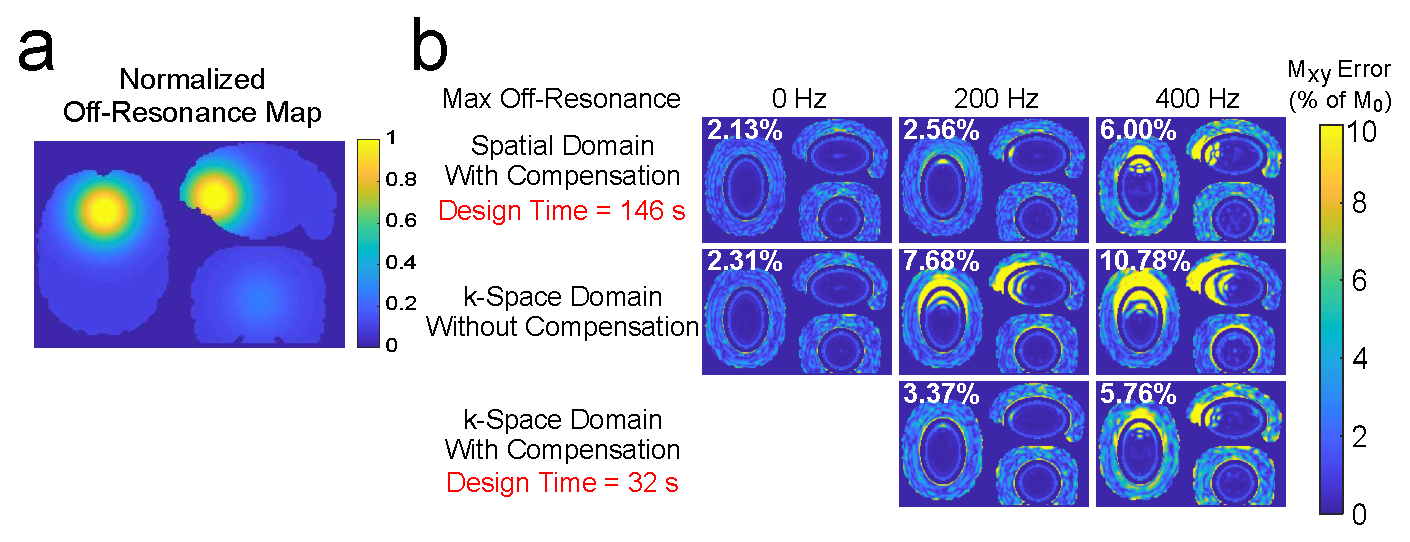
\includegraphics[width=\textwidth]{OffResonance}
	\caption{
	(a) Normalized off-resonance map containing a Gaussian distortion centered above the frontal sinus, 
	to mimic air-tissue susceptibility difference-induced $B_0$ inhomogeneity.
	(b) Normalized excitation maps and RMSEs for spatial domain design with off-resonance correction (first row), 
	and k-space domain design without and with off-resonance correction (second and third rows).}
	\label{fig:kspace_PTX_B0}
\end{figure}

Regarding 3D off-resonance patterns with the shape shown in Figure \ref{fig:kspace_PTX_B0}a and different scaling, Figure \ref{fig:kspace_PTX_B0}b shows the excitation maps of three types of designs: spatial domain design with off-resonance correction (first row), k-space domain design with and without off-resonance correction (second \& third row). As shown in the second row of Figure \ref{fig:kspace_PTX_B0}b, off-resonance caused false excitation outside the designated suppression region, and must be corrected. With 200 Hz maximum off-resonance, which is the typical range of off-resonance observed in clinical studies, k-space domain design with correction was able to fully correct the off-resonance artifacts. It was also able to provide excitation pattern comparable to spatial domain design with 400 Hz maximum off-resonance. The k-space domain design has a weaker performance with higher off-resonance due to the fact that the time segmentation approximation in Ref \cite{fessler2005toeplitz} was meant to approximate forward models from RF to excitation patterns and does not serve as an accurate approximation to the backward model as we need in the k-space domain design.